% To compile single chapters put a % symbol in front of "\comment" and "}%end of comment" below 
%    and take off the % symbol from "\end{document" at the bottom line. Undo before compiling
%    the complete thesis
%%Note: You can only use \section command, you are not allowed, per TTU Graduate School, use
%%\subsection command for ghigher level subheadings. At most level 2 subheadings are allowed.

\chapter{Anomaly Detection Systems}
\label{Anomaly Detection Systems Chapter}

\section[Data Requirements]{Data Set Requirements}

To ascertain the ability of the DASP algorithms and subsequent image processing, feature extraction, and machine learning algorithms to characterize and classify devices based upon their respective URE, a data set of sufficient size and diversity was required to provide reliable statistics and performance metrics.  Table \ref{tab:collection_requirements} outlines the self-imposed URE collection system and device requirements for a data set suitable for evaluation of the DASP algorithms.  No publicly available data sets were identified that met the criteria for evaluation of the DASP algorithms, with the vast majority being too low in sample rate ($< 15$kHz), such as Smart* \cite{Barker2012}, AMPds \cite{Makonin2013}, BLUED \cite{Filip2011}, ECO \cite{Beckel2014}, and iAWE \cite{Batra2014}.  In addition, existing data sets also tended to focus on large appliances or whole house measurements as with the REDD \cite{Kolter2011},  Plaid \cite{Gao2014}, and UK-DALE \cite{Kelly2015}, as opposed to focusing on single measurements of small electronic devices.  \cite{Gulati2014} did provide a high frequency ($>1$Ms/s) data set of EMI signatures from small commercial electronic device, unfortunately the number of data captures per device were not sufficient for the machine learning processing requirements. 

\begin{table}[tb]
	\caption{URE data set collection and device requirements for evaluation of DASP algorithms and their applicability to URE classification.}
	\centering
		\begin{tabular}{c|c}
		\hline
		Metric & Value \\
		\hline
    Sample Rate & $ \ge 1$MS/s\\
		Bits of Resolution & $ \geq 12$ bits \\
		Collection Type & Baseband Measurements Required \\
		Power Line Frequency Filtering & Preferred \\
		Number of Devices & $\geq 10$ Devices \\
		Number of Measurements & $ \geq 100$ per Device\\
		Types of Devices & Consumer Electronic Devices \\
		Measurement of ``Off'' State & Required \\
		Collection Environment & Relatively Low Noise \\
		Ground Truth Documentation & Required \\
		Measurement Type & Ground to Neutral Voltage Preferred \\
		& Ground or Neutral Current Probe Acceptable \\
    \hline
		\end{tabular}
	\label{tab:collection_requirements}
\end{table}

Although many of the constraints in Table \ref{tab:collection_requirements} are self-evident, several were refined through the initial collection and DASP test and evaluation phases.  For instance, early testing showed significant spectral content at frequencies greater than $100$kHz for several devices, as also identified by \cite{Gulati2014}, and therefore a higher sampling rate greater than or equal to $1$MS/s was desired.   In addition, URE content was identified within current probe captures of the ground and neutral lines as well as voltage measurements between the power line conductors, however a voltage probe measurement was preferred given the ease of installation and potential utilization in commercial and residential applications.

\section[Collection Setup]{Collection Setup}

Due to the inability to identify a suitable data set for DASP processing, a collection system was developed and consumer electronic devices gathered to satisfy the requirements set forth in Table \ref{tab:collection_requirements}.  The URE signal captures were performed in a radio frequency (RF) shielded enclosure using a Universal Software Radio Peripheral (USRP) N210 collection platform with an LFRX analog-to-digital processing board operating at $2$MS/s.  The conducted URE signals were measured using a high impedance differential voltage probe between the ground and neutral conductors providing power to the RF chamber, as pictured in Figure \ref{fig:chamber_pic}.  A Twin-T high-pass filter \cite{Cooke2016} was installed in series with the high impedance voltage probe, as shown in Figure \ref{fig:twint_filter_schematic}, to reduce the $60$Hz power line frequency and maximize the dynamic range of the system.  The voltage attenuation response versus frequency is shown in Figure \ref{fig:twint_filter_response}.

\begin{figure}[tb]
	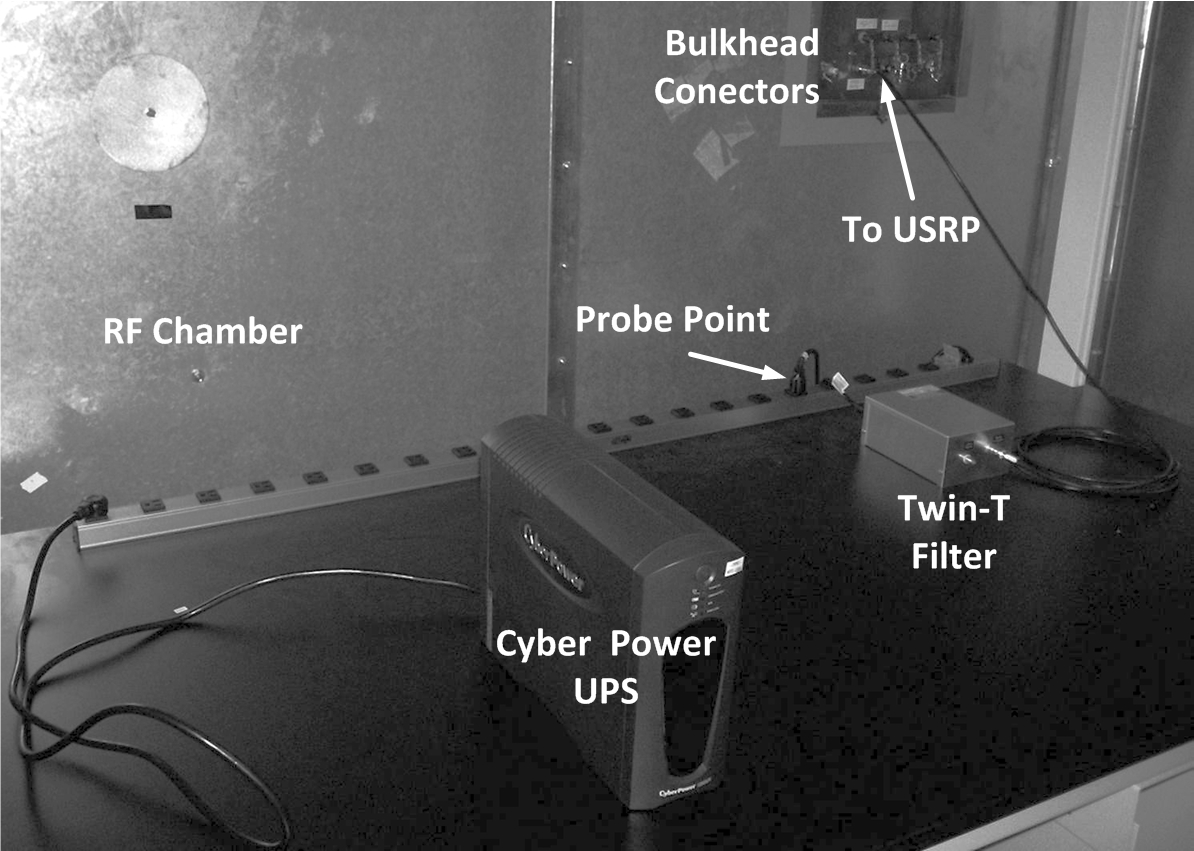
\includegraphics[width=\textwidth]{./data_collection_results/chamberAdj.jpg}
	\centering
	\caption{Picture of URE signal collection being performed on the \textit{cyberpowerups} device.  URE collection was conducted within an RF shielded enclosure with the filtered differential probe signal relayed to an external collection system through an RF bulkhead connection.}
	\label{fig:chamber_pic}
\end{figure}

\begin{figure}[tb]
	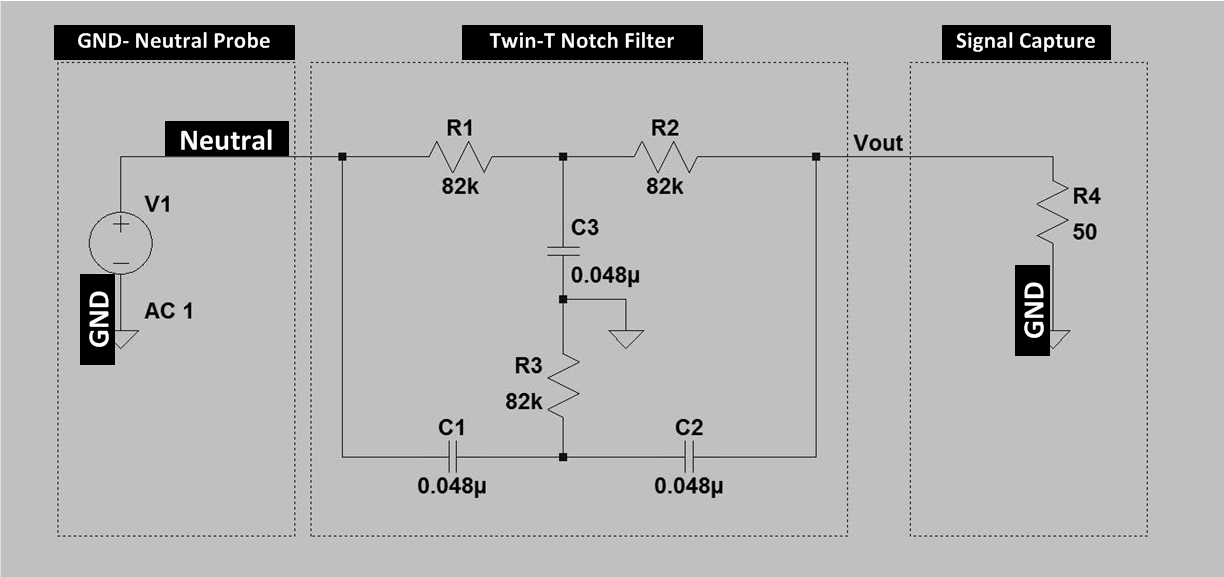
\includegraphics[width=\textwidth]{./data_collection_results/filter_schematic}
	\centering
	\caption{Schematic of Twin-T notch filter used for filtering the $60$Hz power line frequency.  The conducted URE signal sampling was performed with a differential measurement between the power line neutral and ground, with sampling performed by a USRP N210.}
	\label{fig:twint_filter_schematic}
\end{figure}

\begin{figure}[tb]
	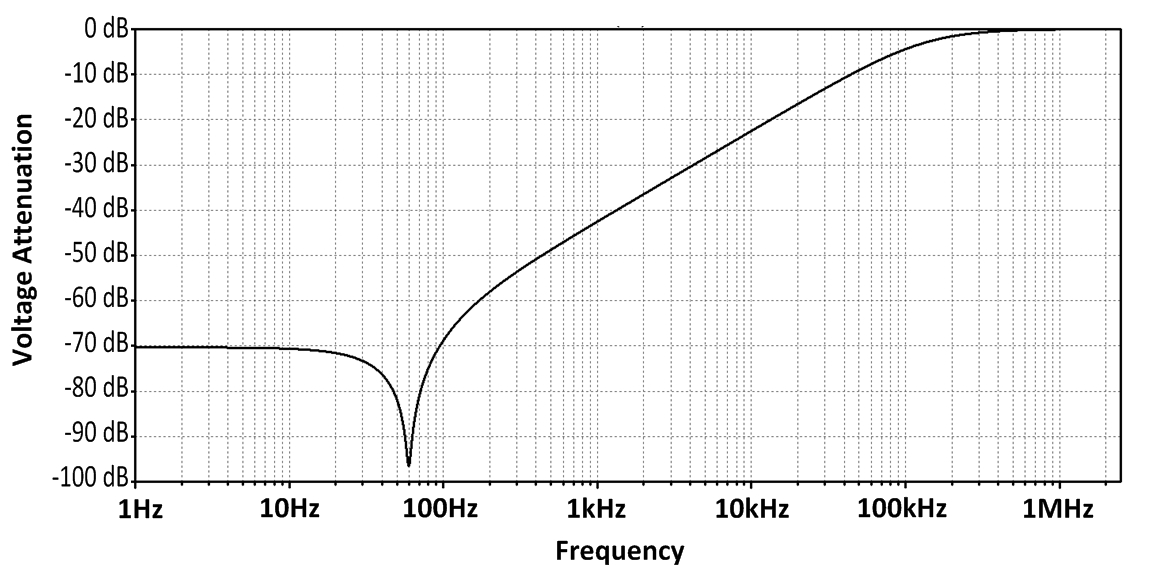
\includegraphics[width=\textwidth]{./data_collection_results/filter_response.jpg}
	\centering
	\caption{Twin-T voltage attenuation response versus frequency.  The filter was designed to provide a greater than $50$dB voltage attenuation to the power line frequency and its first harmonic ($60$Hz and $120$Hz) \cite{Cooke2016}.}
	\label{fig:twint_filter_response}
\end{figure}

The USRP N210 was equipped with a temperature-compensated crystal oscillator (TCXO) which provided a $2.5$ parts-per-million (ppm) frequency accuracy.  Although the TCXO did not provide the temperature stability of oven-controlled or GPS disciplined oscillators, the lower cost, size, and power requirements of the TCXO provided a viable basis for low cost commercial applications.  To further demonstrate commercial applicability, no effort was made to calibrate or quantify the frequency stability of the USRP N210 collection system.

\section[Test Devices]{Test Devices}

Twenty-one commercially available consumer electronic devices were selected for URE collection in the RF shielded enclosure.  The devices were selected to represent a typical home and office environment, with class types ranging from computing platforms to gaming systems to media players.  The devices, along with the inclusion of the \textit{None} state, were separated in to two data sets to represent ``known'' devices for ``Testing and Training'' and ``Unknown'' devices for ``Clutter'' analysis as shown in Table \ref{tab:collection_devices}, where the class names and class descriptions are provided for each device.  Pictures of the ``Test and Training'' devices are shown in Figure \ref{fig:device_pics} as they were positioned in the RF enclosure during the URE collection process.

\begin{table}[tb]
	\caption{A listing of all of the commercial devices utilized for the collection of conducted URE.  Devices were divided between ``Test and Training'' and ``	Clutter''.  In addition to the ``None'' class, the ``Test and Training'' devices were utilized for the majority of analysis, whereas the ``Clutter'' devices were used for clutter analysis as presented in Chapter \ref{DASP Device Classification Chapter}.}
	\centering
		\begin{tabular}{cc|cc}
		\hline
		\multicolumn{2}{c}{Test and Training Devices} & \multicolumn{2}{c}{Clutter Devices} \\
		Description & Name & Description & Name\\
		\hline
    None & None & BluRay Player & viziobluray \\
		UPS & cyberpowerups & Desk Phone & cortelphone \\
		Monitor & dellmonitor & Desk Phone & lgphone \\
		Desktop & delloptiplex & Single Board Computer & odroidxu4 \\
		Desktop & dellxps & VOIP Phone & polycomvoip \\
		Light & fluorescentlights & Single Board Computer & raspberrypi \\
		Printer & hplaserjet & Media Player & roku2xs \\
		Laptop & hpzbook & Single Board Computer & usrpe310 \\
		Router & linksysrouter & Gaming System & vtechvsmile \\
		Monitor & viewsonicmonitor & Gaming System & wiiu\\
		& & Gaming System & xboxone\\
    \hline
		\end{tabular}

	\label{tab:collection_devices}
\end{table}

\begin{figure}[tb]
	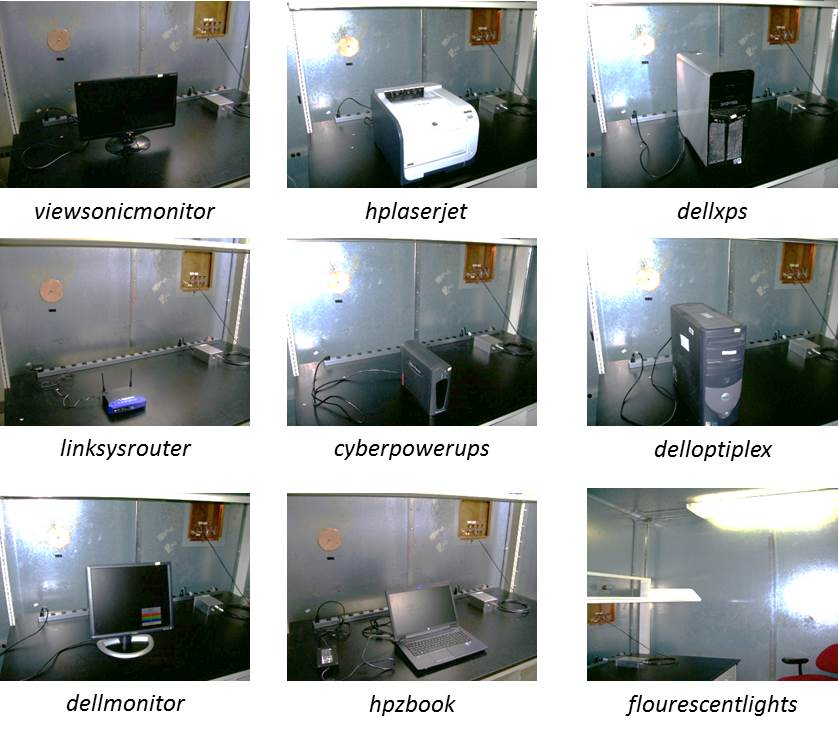
\includegraphics[width=\textwidth]{./data_collection_results/device_pics.jpg}
	\centering
	\caption{Testing and training devices shown in the RF enclosure before collection of URE was conducted.}
	\label{fig:device_pics}
\end{figure}

\section[Collection Process]{Collection Process}

To minimize the noise and confounders in the URE data sets, the devices of interest were placed in an RF shielded enclosure with a power line filtering system.  The collection system was placed outside of the RF shielded enclosure while being fed via a bulkhead connection to the voltage probe within the enclosure.  During collection periods, all electrical devices within the enclosure were powered down except for the device under test.  A set of fluorescent lights was installed in the enclosure and were also turned off during collection periods, except during collection of the \textit{fluorescentlights} device class.  

Collection periods were divided into four $10$ minute segments with the device turned on for the first and third segments and the device unplugged for the second and fourth segments.  Each $10$ minute time domain capture was subsequently divided into contiguous one second capture files resulting in a total of $1200$ time domain captures per device and  $24000$ ``off state'' captures, with each one second time domain capture stored in a MATLAB\textsuperscript \textregistered ~ \textit{.mat} file structure with the fields shown in Table \ref{tab:collection_parameters}.  To allow for software boot-up time and to ensure steady-state operation, a minimum wait period of one minute was provided after the devices were powered on and before signal captures were started.  Additionally, no specific process for exercising the devices under test was conducted, such as playing a Blu-Ray disk or running a specific software application, and furthermore, no provisions were made to prevent a device from entering a low-power or sleep mode during the $10$ minute collection windows.

\begin{table}[tb]
	\caption{Table of recorded fields for each URE collection sample.  In addition to the raw data (\textit{data}), the collection conditions, device information, and collection time are all recorded.}
	\centering
		\begin{tabular}{c|c|c}
		\hline
		Field Name & Description & Example \\
		\hline
    \textit{data} & Time domain sampled signal & $1 \times 200000$ int16 vector \\
		\textit{samp\_rate} & Sample Rate & $2000000$ \\
		\textit{meastype} & Voltage probe configuration & \textit{ng} (i.e Neutral to Ground) \\
		\textit{devclass} & Class of Device & \textit{phone} \\
		\textit{devname} & Name of Device & \textit{cortelphone} \\
		\textit{partnum} & Part Number of Device & \textit{270000 TP2 27S} \\
		\textit{serialnum} & Serial Number of Device & \textit{027046} \\
		\textit{year} & Collection Year & $2016$ \\
		\textit{month} & Collection Month & $6$ \\
		\textit{day} & Collection Day & $24$ \\
		\textit{hour} & Collection Hour & $16$ \\
		\textit{minute} & Collection Minute & $5$ \\
		\textit{second} & Collection Second & $6$ \\
    \hline
		\end{tabular}
	\label{tab:collection_parameters}
\end{table}